\documentclass[border=5pt]{standalone}
\usepackage{tikz}
\usetikzlibrary{matrix}

\begin{document}
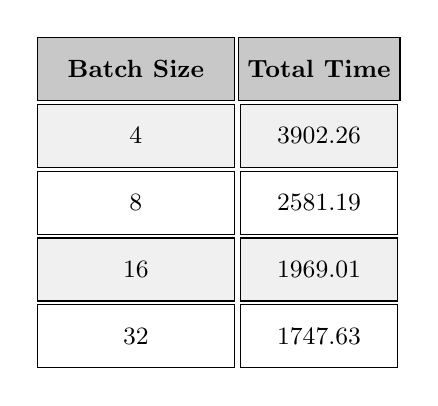
\begin{tikzpicture}

% Define colors for styling
\definecolor{headerColor}{RGB}{200,200,200} % Light gray for header
\definecolor{rowColor1}{RGB}{240,240,240}  % Light gray for odd rows
\definecolor{rowColor2}{RGB}{255,255,255}  % White for even rows

% Create the table using a matrix
\matrix (m) [
  matrix of nodes,
  nodes={
    draw, % Draw borders for each cell
    minimum height=0.8cm, % Height of each cell
    minimum width=2cm, % Width of each cell for most columns
    anchor=center,
    font=\small % Smaller font for readability
  },
  column 1/.style={nodes={minimum width=2.5cm}}, % Wider column for "Batch Size"
  column 7/.style={nodes={minimum width=2.5cm}}, % Wider column for "Total Time"
  row 1/.style={nodes={fill=headerColor, font=\small\bfseries}}, % Style for header row
  row 2/.style={nodes={fill=rowColor1}}, % Style for batch size 4
  row 3/.style={nodes={fill=rowColor2}}, % Style for batch size 8
  row 4/.style={nodes={fill=rowColor1}}, % Style for batch size 16
  row 5/.style={nodes={fill=rowColor2}}, % Style for batch size 32
  column sep=1pt, % Small separation between columns
  row sep=1pt % Small separation between rows
] {
  Batch Size & Total Time \\
  4  & 3902.26 \\
  8  & 2581.19 \\
  16 & 1969.01 \\
  32 & 1747.63 \\
};

\end{tikzpicture}
\end{document}%! Author = Professional
%! Date = 4/24/2025

% Preamble
\documentclass[11pt]{article}

% Packages
\usepackage{amsmath}

% Document
\begin{document}



\end{document}